\documentclass[t, 10pt, handout, aspectratio=169]{beamer}
\usepackage{lipsum}
\usepackage[russian,english]{babel}
\usepackage{tikz}
\usepackage{pgfplots, pgfplotstable}
\usepackage{booktabs}
\usepackage{graphicx}
\pgfplotsset{compat=1.14}
\usetheme[color=blue,framenumber,totalframenumber, footline, footertext]{KU}

\title[]{Лекция 1}
\subtitle{Перевод из одной СС в другую. Пример 1}

\date[30/02/1984]{30 февраля 1984}


\begin{document}
\selectlanguage{russian}

\begin{frame}
  \titlepage
\end{frame}

% \section{My section}
% \subsection{My subsection}

\begin{frame}{Перевод из одной СС в другую}{Пример 2}
  \begin{columns}[2]
    \begin{column}{.5\textwidth}
        \textbf{Задача:} $ 231_{(10)} = \ ?_{(2)} $
        \\[1.2cm]
        % \hspace{1.8cm} 
        Ход решения →
        \\[1.2cm]
        \textbf{Ответ:} $231_{(10)} = 11100111_{(2)}$
    \end{column}
    \begin{column}{.5\textwidth}
        % \includegraphics[<options, e.g. width=\textwidth>]{<your image file>}
        \vspace{-0.5cm}
        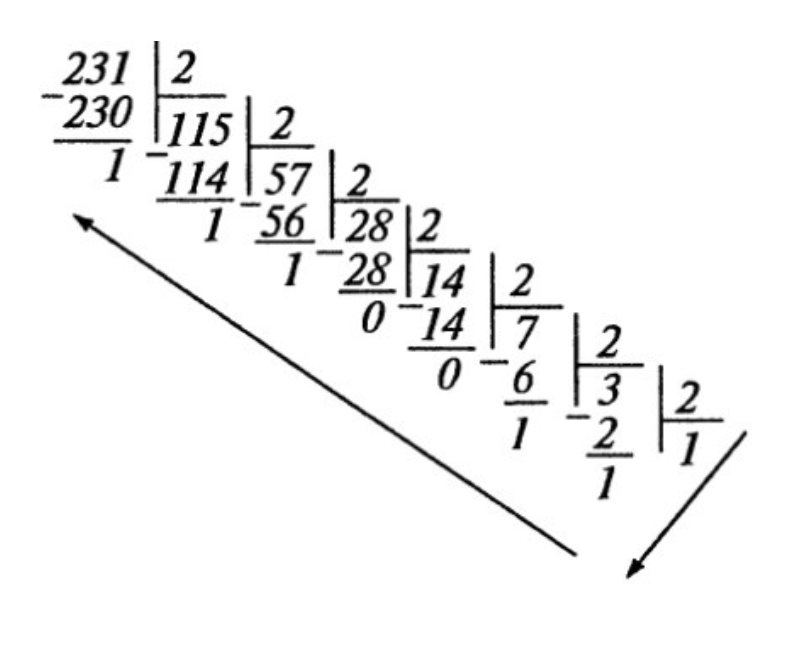
\includegraphics[width=\textwidth, scale=0.4]{logos/division_inf.png}
    \end{column}
  \end{columns}
\end{frame}

\begin{frame}{Перевод из одной СС в другую}{Пример 4}
  \begin{columns}[2]
    \begin{column}{.7\textwidth}
        % \vspace{-2cm}
        % \ \\
        \textbf{Задача:} $ 0.8125_{(10)} = \ ?_{(2)} $
        \\[1.2cm]
        % \hspace{1.8cm} 
        Ход решения →
        \\[1.2cm]
        \textbf{Ответ:} $0.8125_{(10)} = 1*2^{-1} +1*2^{-2} +1*2^{-4} = 0.1101_{(2)}$
    \end{column}
    \begin{column}{0.3\textwidth}
        % \includegraphics[<options, e.g. width=\textwidth>]{<your image file>}
        \vspace{-1.9cm}
        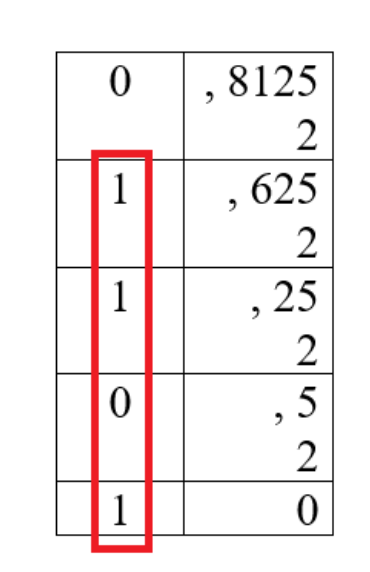
\includegraphics[width=\textwidth, scale=0.4]{logos/table_frac_inf.png}
    \end{column}
  \end{columns}
\end{frame}


\begin{frame}
  \frametitle{Преобразование из CC-N в CC-N\textsuperscript{k} и обратно}
  % \vspace{-5pt}
  {\large{Из СС-N в СС-N\textsuperscript{k}}}
  \vspace{-2pt}
  \begin{itemize}%[leftmargin=0pt]
      \item дополнить число, записанное в СС с основанием N, незначащими нулями так, чтобы количество цифр было кратно k;
      \item разбить полученное число на группы по k цифр, начиная от нуля;
      \item заменить каждую такую группу эквивалентным числом, записанным в СС с основанием N\textsuperscript{k}.
  \end{itemize}
  Задача: $1020101_{(3)} = ?_{(27)}$ \\
  Решение: $1020101_{(3)} = 001\ 020\ 101_{(3)} = 16A?_{(27)}$ \\[0.3cm]
  {\large{Из СС-N\textsuperscript{k} в СС-N}}
  \vspace{-2pt}
  \begin{itemize}%[leftmargin=0pt]
      \item заменить каждую цифру числа, записанного в CC с основанием N\textsuperscript{k}, эквивалентным набором из k цифр CC с основанием N.
  \end{itemize}
  Задача: $2345_{(125)} = ?_{(5)}$ \\
  Решение: $2345_{(125)} = 002\ 003\ 004\ 010_{(5)} = 2003004010_{(5)}$
  % \framesubtitle{Из СС-N в СС-N\textsuperscript{k}}
\end{frame}

\begin{frame}
  \frametitle{Оптимальная система счисления}
    \textbf{Задача.} Робинзон Крузо нашёл на острове 60 камней. Сколько прошедших дней можно ими закодировать в разных СС?
    \setlength{\columnsep}{30pt}
    \\[12pt]
    \begin{minipage}[t]{0.25\linewidth}
        \vspace{6pt}
        \textbf{Пример СС-10:}
    \end{minipage}
    \begin{minipage}[t]{0.25\linewidth}
        \vspace{0pt}
        
\includegraphics[width=2cm, scale=0.4]{logos/crusoe_dots1.png}
    \end{minipage}
    \begin{minipage}[t]{0.4\linewidth}
        \vspace{0pt}
        463502-й день из 999999 возможных, где 999999 = 10\textsuperscript{6} - 1 \\[0.3cm]
        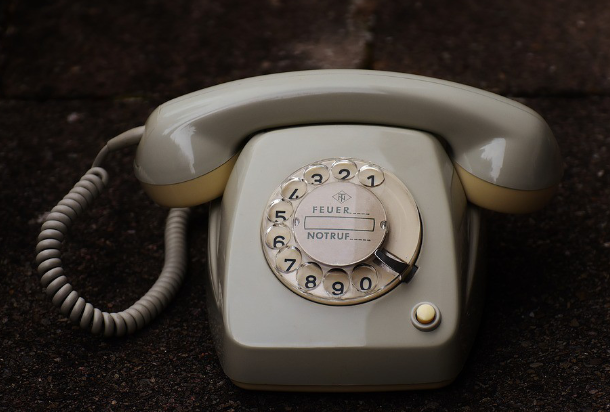
\includegraphics[width=4.6cm, scale=0.4]{logos/iphone20promax.png}
    \end{minipage}
\end{frame}

\begin{frame}
    \frametitle{Оптимальная система счисления (2)}
    \begin{minipage}[t]{0.4\linewidth}
        \vspace{0pt}
        \textbf{Пример СС-10:} \\
        0 камней = 0 дней \\
        1 камень = 1 день \\
        2 камня = 2 дня \\
        ... \\
        \textbf{60 камней} = 60 дней
    \end{minipage}
    \begin{minipage}[t]{0.2\linewidth}
        \vspace{-6pt}
        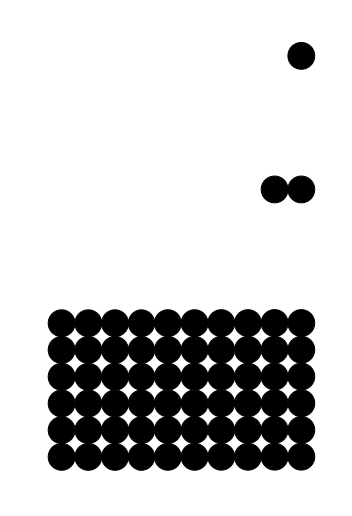
\includegraphics[width=2cm, scale=0.4]{logos/crusoe_dots2.png}
    \end{minipage}
    \begin{minipage}[t]{0.2\linewidth}
        \vspace{0pt}
        1 день \\[0.4cm]
        2 дня \\[0.4cm]
        60 дней
    \end{minipage}
\end{frame}







\end{document}
